% Options for packages loaded elsewhere
\PassOptionsToPackage{unicode}{hyperref}
\PassOptionsToPackage{hyphens}{url}
\PassOptionsToPackage{dvipsnames,svgnames*,x11names*}{xcolor}
%
\documentclass[
  ignorenonframetext,
]{beamer}
\usepackage{pgfpages}
\setbeamertemplate{caption}[numbered]
\setbeamertemplate{caption label separator}{: }
\setbeamercolor{caption name}{fg=normal text.fg}
\beamertemplatenavigationsymbolsempty
% Prevent slide breaks in the middle of a paragraph
\widowpenalties 1 10000
\raggedbottom
\setbeamertemplate{part page}{
  \centering
  \begin{beamercolorbox}[sep=16pt,center]{part title}
    \usebeamerfont{part title}\insertpart\par
  \end{beamercolorbox}
}
\setbeamertemplate{section page}{
  \centering
  \begin{beamercolorbox}[sep=12pt,center]{part title}
    \usebeamerfont{section title}\insertsection\par
  \end{beamercolorbox}
}
\setbeamertemplate{subsection page}{
  \centering
  \begin{beamercolorbox}[sep=8pt,center]{part title}
    \usebeamerfont{subsection title}\insertsubsection\par
  \end{beamercolorbox}
}
\AtBeginPart{
  \frame{\partpage}
}
\AtBeginSection{
  \ifbibliography
  \else
    \frame{\sectionpage}
  \fi
}
\AtBeginSubsection{
  \frame{\subsectionpage}
}
\usepackage{lmodern}
\usepackage{amssymb,amsmath}
\usepackage{ifxetex,ifluatex}
\ifnum 0\ifxetex 1\fi\ifluatex 1\fi=0 % if pdftex
  \usepackage[T1]{fontenc}
  \usepackage[utf8]{inputenc}
  \usepackage{textcomp} % provide euro and other symbols
\else % if luatex or xetex
  \usepackage{unicode-math}
  \defaultfontfeatures{Scale=MatchLowercase}
  \defaultfontfeatures[\rmfamily]{Ligatures=TeX,Scale=1}
\fi
% Use upquote if available, for straight quotes in verbatim environments
\IfFileExists{upquote.sty}{\usepackage{upquote}}{}
\IfFileExists{microtype.sty}{% use microtype if available
  \usepackage[]{microtype}
  \UseMicrotypeSet[protrusion]{basicmath} % disable protrusion for tt fonts
}{}
\makeatletter
\@ifundefined{KOMAClassName}{% if non-KOMA class
  \IfFileExists{parskip.sty}{%
    \usepackage{parskip}
  }{% else
    \setlength{\parindent}{0pt}
    \setlength{\parskip}{6pt plus 2pt minus 1pt}}
}{% if KOMA class
  \KOMAoptions{parskip=half}}
\makeatother
\usepackage{xcolor}
\IfFileExists{xurl.sty}{\usepackage{xurl}}{} % add URL line breaks if available
\IfFileExists{bookmark.sty}{\usepackage{bookmark}}{\usepackage{hyperref}}
\hypersetup{
  pdftitle={Bayesian Statistics},
  pdfauthor={Zack Treisman},
  colorlinks=true,
  linkcolor=Maroon,
  filecolor=Maroon,
  citecolor=blue,
  urlcolor=Blue,
  pdfcreator={LaTeX via pandoc}}
\urlstyle{same} % disable monospaced font for URLs
\newif\ifbibliography
\usepackage{color}
\usepackage{fancyvrb}
\newcommand{\VerbBar}{|}
\newcommand{\VERB}{\Verb[commandchars=\\\{\}]}
\DefineVerbatimEnvironment{Highlighting}{Verbatim}{commandchars=\\\{\}}
% Add ',fontsize=\small' for more characters per line
\usepackage{framed}
\definecolor{shadecolor}{RGB}{248,248,248}
\newenvironment{Shaded}{\begin{snugshade}}{\end{snugshade}}
\newcommand{\AlertTok}[1]{\textcolor[rgb]{0.94,0.16,0.16}{#1}}
\newcommand{\AnnotationTok}[1]{\textcolor[rgb]{0.56,0.35,0.01}{\textbf{\textit{#1}}}}
\newcommand{\AttributeTok}[1]{\textcolor[rgb]{0.77,0.63,0.00}{#1}}
\newcommand{\BaseNTok}[1]{\textcolor[rgb]{0.00,0.00,0.81}{#1}}
\newcommand{\BuiltInTok}[1]{#1}
\newcommand{\CharTok}[1]{\textcolor[rgb]{0.31,0.60,0.02}{#1}}
\newcommand{\CommentTok}[1]{\textcolor[rgb]{0.56,0.35,0.01}{\textit{#1}}}
\newcommand{\CommentVarTok}[1]{\textcolor[rgb]{0.56,0.35,0.01}{\textbf{\textit{#1}}}}
\newcommand{\ConstantTok}[1]{\textcolor[rgb]{0.00,0.00,0.00}{#1}}
\newcommand{\ControlFlowTok}[1]{\textcolor[rgb]{0.13,0.29,0.53}{\textbf{#1}}}
\newcommand{\DataTypeTok}[1]{\textcolor[rgb]{0.13,0.29,0.53}{#1}}
\newcommand{\DecValTok}[1]{\textcolor[rgb]{0.00,0.00,0.81}{#1}}
\newcommand{\DocumentationTok}[1]{\textcolor[rgb]{0.56,0.35,0.01}{\textbf{\textit{#1}}}}
\newcommand{\ErrorTok}[1]{\textcolor[rgb]{0.64,0.00,0.00}{\textbf{#1}}}
\newcommand{\ExtensionTok}[1]{#1}
\newcommand{\FloatTok}[1]{\textcolor[rgb]{0.00,0.00,0.81}{#1}}
\newcommand{\FunctionTok}[1]{\textcolor[rgb]{0.00,0.00,0.00}{#1}}
\newcommand{\ImportTok}[1]{#1}
\newcommand{\InformationTok}[1]{\textcolor[rgb]{0.56,0.35,0.01}{\textbf{\textit{#1}}}}
\newcommand{\KeywordTok}[1]{\textcolor[rgb]{0.13,0.29,0.53}{\textbf{#1}}}
\newcommand{\NormalTok}[1]{#1}
\newcommand{\OperatorTok}[1]{\textcolor[rgb]{0.81,0.36,0.00}{\textbf{#1}}}
\newcommand{\OtherTok}[1]{\textcolor[rgb]{0.56,0.35,0.01}{#1}}
\newcommand{\PreprocessorTok}[1]{\textcolor[rgb]{0.56,0.35,0.01}{\textit{#1}}}
\newcommand{\RegionMarkerTok}[1]{#1}
\newcommand{\SpecialCharTok}[1]{\textcolor[rgb]{0.00,0.00,0.00}{#1}}
\newcommand{\SpecialStringTok}[1]{\textcolor[rgb]{0.31,0.60,0.02}{#1}}
\newcommand{\StringTok}[1]{\textcolor[rgb]{0.31,0.60,0.02}{#1}}
\newcommand{\VariableTok}[1]{\textcolor[rgb]{0.00,0.00,0.00}{#1}}
\newcommand{\VerbatimStringTok}[1]{\textcolor[rgb]{0.31,0.60,0.02}{#1}}
\newcommand{\WarningTok}[1]{\textcolor[rgb]{0.56,0.35,0.01}{\textbf{\textit{#1}}}}
\usepackage{graphicx,grffile}
\makeatletter
\def\maxwidth{\ifdim\Gin@nat@width>\linewidth\linewidth\else\Gin@nat@width\fi}
\def\maxheight{\ifdim\Gin@nat@height>\textheight\textheight\else\Gin@nat@height\fi}
\makeatother
% Scale images if necessary, so that they will not overflow the page
% margins by default, and it is still possible to overwrite the defaults
% using explicit options in \includegraphics[width, height, ...]{}
\setkeys{Gin}{width=\maxwidth,height=\maxheight,keepaspectratio}
% Set default figure placement to htbp
\makeatletter
\def\fps@figure{htbp}
\makeatother
\setlength{\emergencystretch}{3em} % prevent overfull lines
\providecommand{\tightlist}{%
  \setlength{\itemsep}{0pt}\setlength{\parskip}{0pt}}
\setcounter{secnumdepth}{-\maxdimen} % remove section numbering

\pgfdeclareimage[width=3.5cm]{mcslogo}{../western_logo_hor_MCS_3C_pos.pdf}
\pgfdeclareimage[width=1cm]{ccbysa}{../ccbysa88x31.png}
\titlegraphic{\href{http://creativecommons.org/licenses/by-sa/4.0/}{\pgfuseimage{ccbysa}}
\hfill
\href{https://western.edu/program/mathematics/}{\pgfuseimage{mcslogo}}}
%\usecolortheme{wcu}
%\institute{Western Colorado University}
%\setbeamertemplate{navigation symbols}{}

\title{Bayesian Statistics}
\author{Zack Treisman}
\date{Spring 2021}

\begin{document}
\frame{\titlepage}

\begin{frame}{Philosophy}
\protect\hypertarget{philosophy}{}

Bayesian statistics is based on a fairly simple procedure, not
dissimilar to what is done in the non-Bayesian scenario.

\begin{itemize}
\tightlist
\item
  Propose a form for a model. (For example, define a deterministic
  function and a stochastic error distribution.)
\item
  Set probability distributions of parameters of the model based on
  \emph{prior} information. (This is the controversial part.)
\item
  Update the parameter distributions based on data. (This is the part
  that can be computationally challenging.)
\end{itemize}

The initial part of a Bayesian analysis is exactly the same as a
frequentist analysis: Explore the data graphically and numerically, and
come up with appropriate forms for models.

\end{frame}

\begin{frame}{Bayes' Rule}
\protect\hypertarget{bayes-rule}{}

Supposing a model with parameters \(\theta\), and given observed data
\(x\), compute the probability distribution for \(\theta\) conditioned
on the observations \(x\) using Bayes' Rule. \[
P(\theta|x)=\frac{P(x|\theta)P(\theta)}{P(x)}
\] If we consider the data to be fixed, then \(P(x)\) is the same for
all possible models, so if we only want to compare models with different
values of \(\theta\), we can ignore the denominator. \[
P(\theta|x)\propto P(x|\theta)P(\theta)
\] Or, more colloquially: \[
\text{Posterior} \propto \text{Likelihood} \times \text{Prior}
\]

\end{frame}

\begin{frame}[fragile]{Distributions of parameters}
\protect\hypertarget{distributions-of-parameters}{}

A key difference between Bayesian analysis and frequentist analysis is
that the parameters \(\theta\) of the model are not fixed but described
by probability distributions.

\begin{itemize}
\tightlist
\item
  Maximum likelihood estimation (and thus \texttt{lm}, \texttt{glm},
  etc.) selects the
  \emph{mode}\footnote{\emph{Mode} is another word for \emph{local maximum}.}
  of the likelihood.
\item
  A Bayesian point estimate of a parameter is more likely to be the
  \emph{mean} of the posterior distribution.
\end{itemize}

\end{frame}

\begin{frame}{The problem with priors}
\protect\hypertarget{the-problem-with-priors}{}

If a prior distribution has too much information, then it will require a
lot of data to alter the posterior.

For example, suppose that we are quite certain that \(\theta=\theta_0\),
and so we choose a prior \[
Prior(\theta)\sim N(\theta_0,\delta) 
\] with \(\delta\) some very small number. The graph of this
distribution is basically a spike at \(\theta_0\) and approximately zero
everywhere else.

Then for any \(\theta\) that is very different from \(\theta_0\), the
posterior is still going to be approximately zero, and the data won't be
able to change our minds.

\end{frame}

\begin{frame}{Flat or uninformative priors}
\protect\hypertarget{flat-or-uninformative-priors}{}

The solution to this issue is to work with a suitably uninformative
prior.

\begin{itemize}
\tightlist
\item
  A uniform distribution can make a good prior.

  \begin{itemize}
  \tightlist
  \item
    Uniform on what scale?
  \end{itemize}
\end{itemize}

For a flat prior, the posterior distribution is proportional to the
likelihood.

\end{frame}

\begin{frame}{Conjugate priors}
\protect\hypertarget{conjugate-priors}{}

Binary classification is particularly simple with a Bayesian method.

Recall the binomial distribution for \(x\) successes in \(N\) trials
with probability \(p\) of success. \[
P(x|p) = {N\choose x} p^x(1-p)^{N-x}
\] Fixing \(x\) and \(N\) as coming from observed data and thinking of
\(p\) as the variable makes \(N\choose x\) a constant.

Previous observation of \(s\) successes and \(r\) failures would lead
one to set the prior \(P(p)\) to follow a Beta distribution, which takes
a similar form: \[
P(p)\propto p^s(1-p)^r
\] Thus, by Bayes' rule: \[
P(p|x) \propto p^{x+s}(1-p)^{N-x+r}
\] the posterior is another Beta distribution.

\end{frame}

\begin{frame}{Tadpole predation}
\protect\hypertarget{tadpole-predation}{}

In the subset of the tadpole data we looked at last week, there were 30
out of 40 tadpoles that survived the experiment.

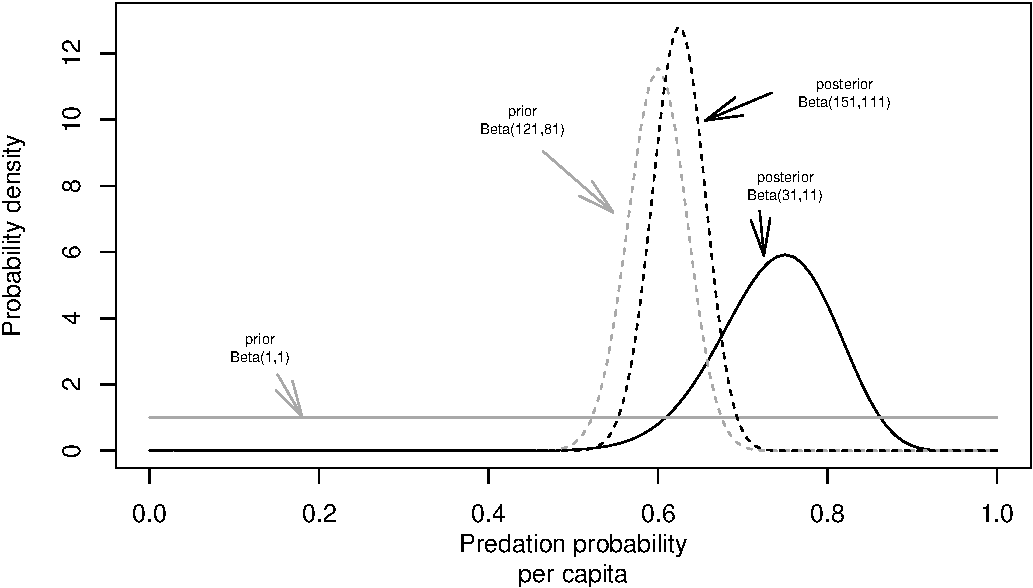
\includegraphics{intro_Bayes_files/figure-beamer/unnamed-chunk-2-1.pdf}

Figure 6.3 from Bolker (2008).

\end{frame}

\begin{frame}{Some things to note}
\protect\hypertarget{some-things-to-note}{}

\begin{itemize}
\item
  With a flat prior, the posterior has mode equal to the maximum
  likelihood estimate. The mean is shifted slightly towards the mean of
  the prior.

  \begin{itemize}
  \tightlist
  \item
    Mode of Beta(31,11) is \((31-1)/(31+11-2)=0.75\).
  \item
    Mean of Beta(31,11) is \(31/(31+11)=0.738\).
  \end{itemize}
\item
  Having a conjugate prior like Binomial/ Beta can make the math easy
  but is not typical, and there are problems that can arise with some
  conjugate priors.
\item
  One big experiment or many small experiments? Doesn't matter. The
  posterior can be updated one observation at a time if we want.
\end{itemize}

\end{frame}

\begin{frame}[fragile]{Bayesian tools in R}
\protect\hypertarget{bayesian-tools-in-r}{}

Many options. Bayesian Regression Models with
Stan\footnote{Stan is a program outside of R that does the computational heavy lifting.}
(\texttt{brms}) seems good. See Bürkner (2018).

Start by fitting an error only (null) model for the tadpole data. Be
warned, Bayesian computations can take some time.

\scriptsize

\begin{Shaded}
\begin{Highlighting}[]
\NormalTok{fit_tad0 <-}\StringTok{ }\KeywordTok{brm}\NormalTok{(surv }\OperatorTok{|}\StringTok{ }\KeywordTok{trials}\NormalTok{(density) }\OperatorTok{~}\StringTok{ }\DecValTok{1}\NormalTok{, }
               \DataTypeTok{family=}\KeywordTok{binomial}\NormalTok{(), }\DataTypeTok{data=}\NormalTok{ReedfrogPred)}
\end{Highlighting}
\end{Shaded}

\begin{Shaded}
\begin{Highlighting}[]
\KeywordTok{summary}\NormalTok{(fit_tad0)}
\end{Highlighting}
\end{Shaded}

\begin{verbatim}
##  Family: binomial 
##   Links: mu = logit 
## Formula: surv | trials(density) ~ 1 
##    Data: ReedfrogPred (Number of observations: 48) 
## Samples: 4 chains, each with iter = 2000; warmup = 1000; thin = 1;
##          total post-warmup samples = 4000
## 
## Population-Level Effects: 
##           Estimate Est.Error l-95% CI u-95% CI Rhat Bulk_ESS Tail_ESS
## Intercept     0.85      0.06     0.73     0.97 1.00     1662     1682
## 
## Samples were drawn using sampling(NUTS). For each parameter, Bulk_ESS
## and Tail_ESS are effective sample size measures, and Rhat is the potential
## scale reduction factor on split chains (at convergence, Rhat = 1).
\end{verbatim}

\end{frame}

\begin{frame}[fragile]{Plot}
\protect\hypertarget{plot}{}

\scriptsize

\begin{Shaded}
\begin{Highlighting}[]
\KeywordTok{plot}\NormalTok{(fit_tad0)}
\end{Highlighting}
\end{Shaded}

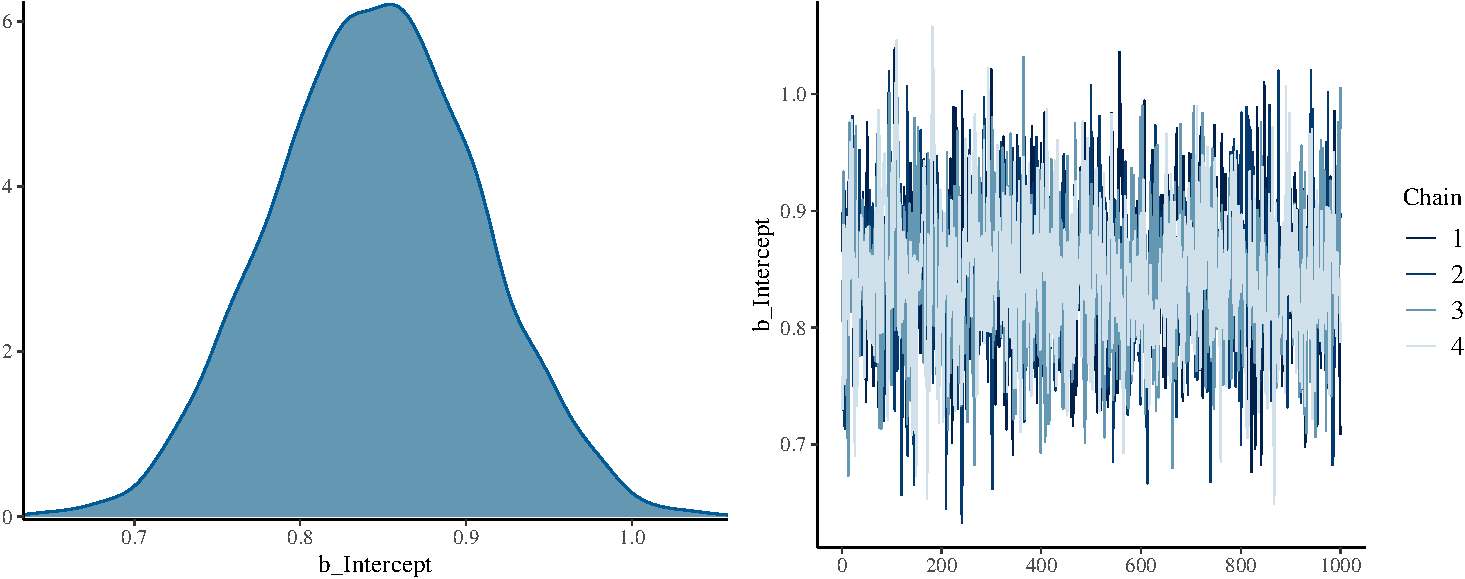
\includegraphics{intro_Bayes_files/figure-beamer/unnamed-chunk-5-1.pdf}

\normalsize

This plot shows a density estimate for the model parameter, and a
diagnostic graph of the convergence of the algorithm used to arrive at
that estimate. The graph on the right indicates a problem if it looks
like anything but random noise.

\end{frame}

\begin{frame}[fragile]{Accessing model parameters}
\protect\hypertarget{accessing-model-parameters}{}

\begin{itemize}
\tightlist
\item
  The coefficients of the \texttt{brm} object are accessed with
  \texttt{\$fixed}.
\end{itemize}

\scriptsize

\begin{Shaded}
\begin{Highlighting}[]
\KeywordTok{summary}\NormalTok{(fit_tad0)}\OperatorTok{$}\NormalTok{fixed}
\end{Highlighting}
\end{Shaded}

\begin{verbatim}
##            Estimate  Est.Error  l-95% CI  u-95% CI     Rhat Bulk_ESS Tail_ESS
## Intercept 0.8458727 0.06239771 0.7260189 0.9686483 1.002481     1662     1682
\end{verbatim}

\normalsize

\begin{itemize}
\tightlist
\item
  The intercept can be converted to a probability with the inverse link
  function.
\end{itemize}

\scriptsize

\begin{Shaded}
\begin{Highlighting}[]
\KeywordTok{plogis}\NormalTok{(}\KeywordTok{summary}\NormalTok{(fit_tad0)}\OperatorTok{$}\NormalTok{fixed[}\DecValTok{1}\NormalTok{])}
\end{Highlighting}
\end{Shaded}

\begin{verbatim}
## [1] 0.6997006
\end{verbatim}

\normalsize

\begin{itemize}
\tightlist
\item
  As expected, this is the overall probability of survival in the data.
\end{itemize}

\scriptsize

\begin{Shaded}
\begin{Highlighting}[]
\KeywordTok{sum}\NormalTok{(ReedfrogPred}\OperatorTok{$}\NormalTok{surv)}\OperatorTok{/}\KeywordTok{sum}\NormalTok{(ReedfrogPred}\OperatorTok{$}\NormalTok{density)}
\end{Highlighting}
\end{Shaded}

\begin{verbatim}
## [1] 0.6991071
\end{verbatim}

\end{frame}

\begin{frame}[fragile]{Set an informative prior}
\protect\hypertarget{set-an-informative-prior}{}

We can impose an informative prior, say of a 75\% survival rate.

\begin{itemize}
\tightlist
\item
  Convert 75\% to the model scale using the link function.
\end{itemize}

\scriptsize

\begin{Shaded}
\begin{Highlighting}[]
\KeywordTok{qlogis}\NormalTok{(}\FloatTok{0.75}\NormalTok{)}
\end{Highlighting}
\end{Shaded}

\begin{verbatim}
## [1] 1.098612
\end{verbatim}

\normalsize

\begin{itemize}
\tightlist
\item
  Because \texttt{brm} creates code that is compiled outside of R, this
  number has to be included explicitly in the prior.
\end{itemize}

\scriptsize

\begin{Shaded}
\begin{Highlighting}[]
\NormalTok{fit_tad0_prior <-}\StringTok{ }\KeywordTok{brm}\NormalTok{(surv }\OperatorTok{|}\StringTok{ }\KeywordTok{trials}\NormalTok{(density) }\OperatorTok{~}\StringTok{ }\DecValTok{1}\NormalTok{, }
                      \DataTypeTok{family=}\KeywordTok{binomial}\NormalTok{(), }\DataTypeTok{data=}\NormalTok{ReedfrogPred, }
                      \DataTypeTok{prior =} \KeywordTok{set_prior}\NormalTok{(}\StringTok{"normal(1.098612,0.1)"}\NormalTok{, }
                                        \DataTypeTok{class =} \StringTok{"Intercept"}\NormalTok{))}
\end{Highlighting}
\end{Shaded}

\begin{Shaded}
\begin{Highlighting}[]
\KeywordTok{plot}\NormalTok{(fit_tad0_prior)}
\end{Highlighting}
\end{Shaded}

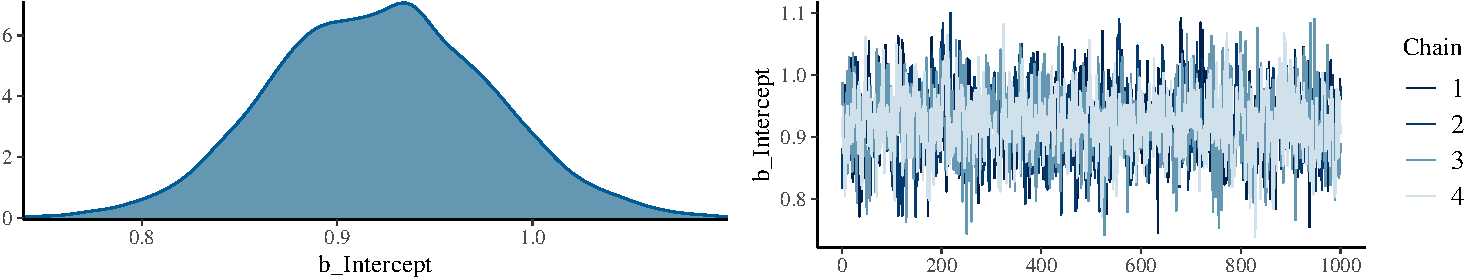
\includegraphics{intro_Bayes_files/figure-beamer/unnamed-chunk-11-1.pdf}

\end{frame}

\begin{frame}[fragile]{A model with predictors}
\protect\hypertarget{a-model-with-predictors}{}

\scriptsize

\begin{Shaded}
\begin{Highlighting}[]
\NormalTok{fit_tad <-}\StringTok{ }\KeywordTok{brm}\NormalTok{(surv }\OperatorTok{|}\StringTok{ }\KeywordTok{trials}\NormalTok{(density) }\OperatorTok{~}\StringTok{ }\NormalTok{pred }\OperatorTok{+}\StringTok{ }\NormalTok{size, }
               \DataTypeTok{family=}\KeywordTok{binomial}\NormalTok{(), }\DataTypeTok{data=}\NormalTok{ReedfrogPred)}
\end{Highlighting}
\end{Shaded}

\begin{Shaded}
\begin{Highlighting}[]
\KeywordTok{summary}\NormalTok{(fit_tad)}
\end{Highlighting}
\end{Shaded}

\begin{verbatim}
##  Family: binomial 
##   Links: mu = logit 
## Formula: surv | trials(density) ~ pred + size 
##    Data: ReedfrogPred (Number of observations: 48) 
## Samples: 4 chains, each with iter = 2000; warmup = 1000; thin = 1;
##          total post-warmup samples = 4000
## 
## Population-Level Effects: 
##           Estimate Est.Error l-95% CI u-95% CI Rhat Bulk_ESS Tail_ESS
## Intercept     2.93      0.19     2.57     3.31 1.00     2062     2110
## predpred     -2.71      0.18    -3.07    -2.36 1.00     2272     2654
## sizebig      -0.67      0.15    -0.98    -0.38 1.00     2979     2657
## 
## Samples were drawn using sampling(NUTS). For each parameter, Bulk_ESS
## and Tail_ESS are effective sample size measures, and Rhat is the potential
## scale reduction factor on split chains (at convergence, Rhat = 1).
\end{verbatim}

\end{frame}

\begin{frame}[fragile]{Plot \texttt{brm} output}
\protect\hypertarget{plot-brm-output}{}

\scriptsize

\begin{Shaded}
\begin{Highlighting}[]
\KeywordTok{plot}\NormalTok{(fit_tad)}
\end{Highlighting}
\end{Shaded}

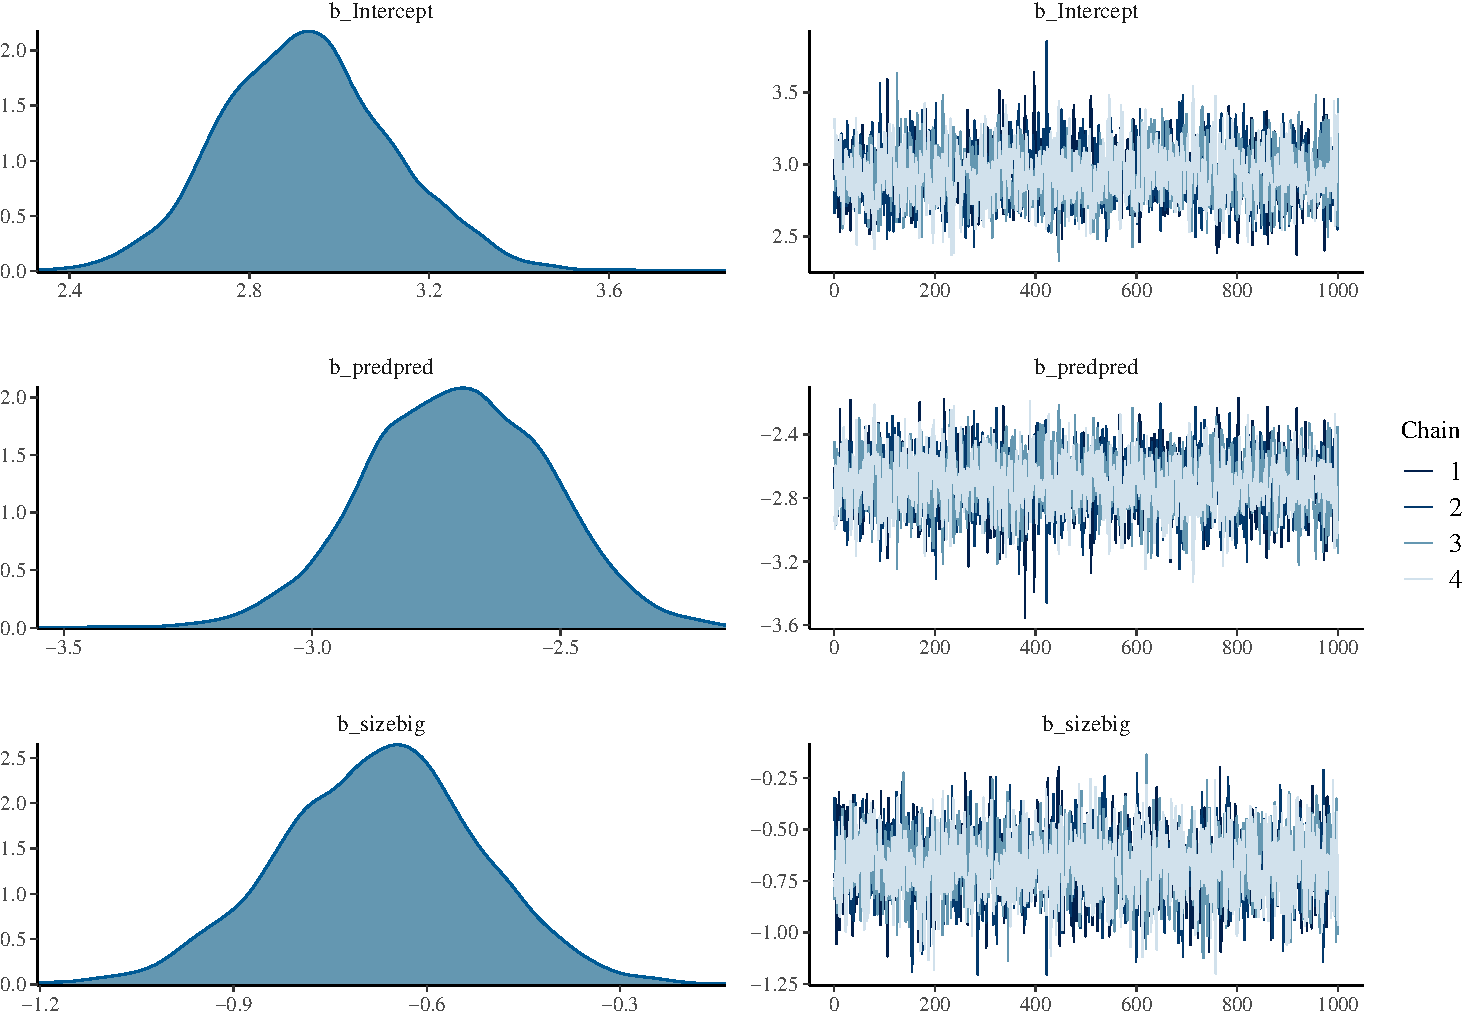
\includegraphics{intro_Bayes_files/figure-beamer/unnamed-chunk-14-1.pdf}

\end{frame}

\begin{frame}[fragile]{The \texttt{brm} with an uninformative prior is
close to a \texttt{glm}}
\protect\hypertarget{the-brm-with-an-uninformative-prior-is-close-to-a-glm}{}

\scriptsize

\begin{Shaded}
\begin{Highlighting}[]
\KeywordTok{summary}\NormalTok{(fit_tad)}\OperatorTok{$}\NormalTok{fixed[,}\DecValTok{1}\OperatorTok{:}\DecValTok{4}\NormalTok{]}
\end{Highlighting}
\end{Shaded}

\begin{verbatim}
##             Estimate Est.Error   l-95% CI   u-95% CI
## Intercept  2.9279091 0.1882503  2.5743609  3.3119765
## predpred  -2.7081062 0.1825929 -3.0693010 -2.3593588
## sizebig   -0.6733214 0.1547661 -0.9814715 -0.3789356
\end{verbatim}

\begin{Shaded}
\begin{Highlighting}[]
\KeywordTok{plogis}\NormalTok{(}\KeywordTok{summary}\NormalTok{(fit_tad)}\OperatorTok{$}\NormalTok{fixed[}\StringTok{"Intercept"}\NormalTok{, }\StringTok{"Estimate"}\NormalTok{])}
\end{Highlighting}
\end{Shaded}

\begin{verbatim}
## [1] 0.949209
\end{verbatim}

\begin{Shaded}
\begin{Highlighting}[]
\KeywordTok{exp}\NormalTok{(}\KeywordTok{summary}\NormalTok{(fit_tad)}\OperatorTok{$}\NormalTok{fixed[,}\StringTok{"Estimate"}\NormalTok{])}
\end{Highlighting}
\end{Shaded}

\begin{verbatim}
##   Intercept    predpred     sizebig 
## 18.68851334  0.06666293  0.51001180
\end{verbatim}

\begin{Shaded}
\begin{Highlighting}[]
\NormalTok{glm_fit_tad <-}\StringTok{ }\KeywordTok{glm}\NormalTok{(}\KeywordTok{cbind}\NormalTok{(surv, density}\OperatorTok{-}\NormalTok{surv) }\OperatorTok{~}\StringTok{ }\NormalTok{pred }\OperatorTok{+}\StringTok{ }\NormalTok{size, }
                   \DataTypeTok{family =} \KeywordTok{binomial}\NormalTok{(), }\DataTypeTok{data =}\NormalTok{ ReedfrogPred)}
\KeywordTok{coef}\NormalTok{(}\KeywordTok{summary}\NormalTok{(glm_fit_tad))}
\end{Highlighting}
\end{Shaded}

\begin{verbatim}
##               Estimate Std. Error    z value     Pr(>|z|)
## (Intercept)  2.9231663  0.1901078  15.376358 2.358447e-53
## predpred    -2.7039259  0.1854929 -14.576976 3.935674e-48
## sizebig     -0.6738492  0.1532298  -4.397639 1.094349e-05
\end{verbatim}

\end{frame}

\begin{frame}[fragile]{Set an informative prior}
\protect\hypertarget{set-an-informative-prior-1}{}

Priors can be set on many parameters of the model. \scriptsize

\begin{Shaded}
\begin{Highlighting}[]
\NormalTok{fit_tad_prior <-}\StringTok{ }\KeywordTok{brm}\NormalTok{(surv }\OperatorTok{|}\StringTok{ }\KeywordTok{trials}\NormalTok{(density) }\OperatorTok{~}\StringTok{ }\NormalTok{pred }\OperatorTok{+}\StringTok{ }\NormalTok{size, }
                     \DataTypeTok{family=}\KeywordTok{binomial}\NormalTok{(), }\DataTypeTok{data=}\NormalTok{ReedfrogPred, }
                     \DataTypeTok{prior =} \KeywordTok{set_prior}\NormalTok{(}\StringTok{"normal(-1,0.1)"}\NormalTok{, }
                                       \DataTypeTok{class =} \StringTok{"b"}\NormalTok{, }
                                       \DataTypeTok{coef =} \StringTok{"sizebig"}\NormalTok{))}
\end{Highlighting}
\end{Shaded}

\begin{Shaded}
\begin{Highlighting}[]
\KeywordTok{summary}\NormalTok{(fit_tad_prior)}
\end{Highlighting}
\end{Shaded}

\begin{verbatim}
##  Family: binomial 
##   Links: mu = logit 
## Formula: surv | trials(density) ~ pred + size 
##    Data: ReedfrogPred (Number of observations: 48) 
## Samples: 4 chains, each with iter = 2000; warmup = 1000; thin = 1;
##          total post-warmup samples = 4000
## 
## Population-Level Effects: 
##           Estimate Est.Error l-95% CI u-95% CI Rhat Bulk_ESS Tail_ESS
## Intercept     3.08      0.18     2.75     3.43 1.00     1762     2103
## predpred     -2.75      0.19    -3.13    -2.39 1.00     2238     2401
## sizebig      -0.90      0.08    -1.07    -0.73 1.00     2908     2826
## 
## Samples were drawn using sampling(NUTS). For each parameter, Bulk_ESS
## and Tail_ESS are effective sample size measures, and Rhat is the potential
## scale reduction factor on split chains (at convergence, Rhat = 1).
\end{verbatim}

\end{frame}

\begin{frame}[fragile]{A nonlinear model}
\protect\hypertarget{a-nonlinear-model}{}

The \texttt{brm} command will fit nonlinear models, such as the
Myxomatosis example in Section 6.3 of Bolker (2008).

\begin{itemize}
\tightlist
\item
  You have to specify a prior, there's no default. Specify priors for
  nonlinear parameters with \texttt{nlpar}.
\item
  The formula goes inside the function \texttt{bf} (for \texttt{brms}
  formula).
\item
  Parameters of the nonlinear function are defined by formulas.
\item
  Set \texttt{nl=TRUE} (for nonlinear).
\end{itemize}

\scriptsize

\begin{Shaded}
\begin{Highlighting}[]
\NormalTok{MyxoTiter_sum}\OperatorTok{$}\NormalTok{fgrade <-}\StringTok{ }\KeywordTok{factor}\NormalTok{(MyxoTiter_sum}\OperatorTok{$}\NormalTok{grade)}
\NormalTok{prior1 <-}\StringTok{ }\KeywordTok{prior}\NormalTok{(}\KeywordTok{normal}\NormalTok{(}\DecValTok{1}\NormalTok{, }\DecValTok{2}\NormalTok{), }\DataTypeTok{nlpar =} \StringTok{"a"}\NormalTok{) }\OperatorTok{+}
\StringTok{  }\KeywordTok{prior}\NormalTok{(}\KeywordTok{normal}\NormalTok{(}\FloatTok{0.2}\NormalTok{, }\FloatTok{0.4}\NormalTok{), }\DataTypeTok{nlpar =} \StringTok{"b"}\NormalTok{) }\OperatorTok{+}\StringTok{ }
\StringTok{  }\KeywordTok{prior}\NormalTok{(}\KeywordTok{gamma}\NormalTok{(}\DecValTok{50}\NormalTok{, }\FloatTok{0.1}\NormalTok{), }\DataTypeTok{class=}\StringTok{"shape"}\NormalTok{)}
\NormalTok{fit_myx <-}\StringTok{ }\KeywordTok{brm}\NormalTok{(}\KeywordTok{bf}\NormalTok{(titer }\OperatorTok{~}\StringTok{ }\NormalTok{a}\OperatorTok{*}\NormalTok{day}\OperatorTok{*}\KeywordTok{exp}\NormalTok{(}\OperatorTok{-}\NormalTok{b}\OperatorTok{*}\NormalTok{day), a}\OperatorTok{~}\NormalTok{fgrade, b}\OperatorTok{~}\NormalTok{fgrade, }\DataTypeTok{nl=}\OtherTok{TRUE}\NormalTok{), }
               \DataTypeTok{data =}\NormalTok{ MyxoTiter_sum, }
               \DataTypeTok{prior =}\NormalTok{ prior1, }
               \DataTypeTok{family=}\KeywordTok{Gamma}\NormalTok{(}\DataTypeTok{link =} \StringTok{"identity"}\NormalTok{))}
\end{Highlighting}
\end{Shaded}

\normalsize

The function we are using, \(\mu_{titer}=a_{g}te^{-b_{g}t}\) is a
reasonable model for a quantity that grows from zero to a peak, and then
decays back to zero.

\end{frame}

\begin{frame}[fragile]{Nonlinear model diagnostic plots}
\protect\hypertarget{nonlinear-model-diagnostic-plots}{}

See \texttt{?plot.brmsfit} or \texttt{?bayesplot} for options. This
model seems to converge okay.

\scriptsize

\begin{Shaded}
\begin{Highlighting}[]
\KeywordTok{plot}\NormalTok{(fit_myx, }\DataTypeTok{pars=}\KeywordTok{c}\NormalTok{(}\StringTok{"b_a_Intercept"}\NormalTok{, }\StringTok{"b_b_Intercept"}\NormalTok{, }\StringTok{"shape"}\NormalTok{))}
\end{Highlighting}
\end{Shaded}

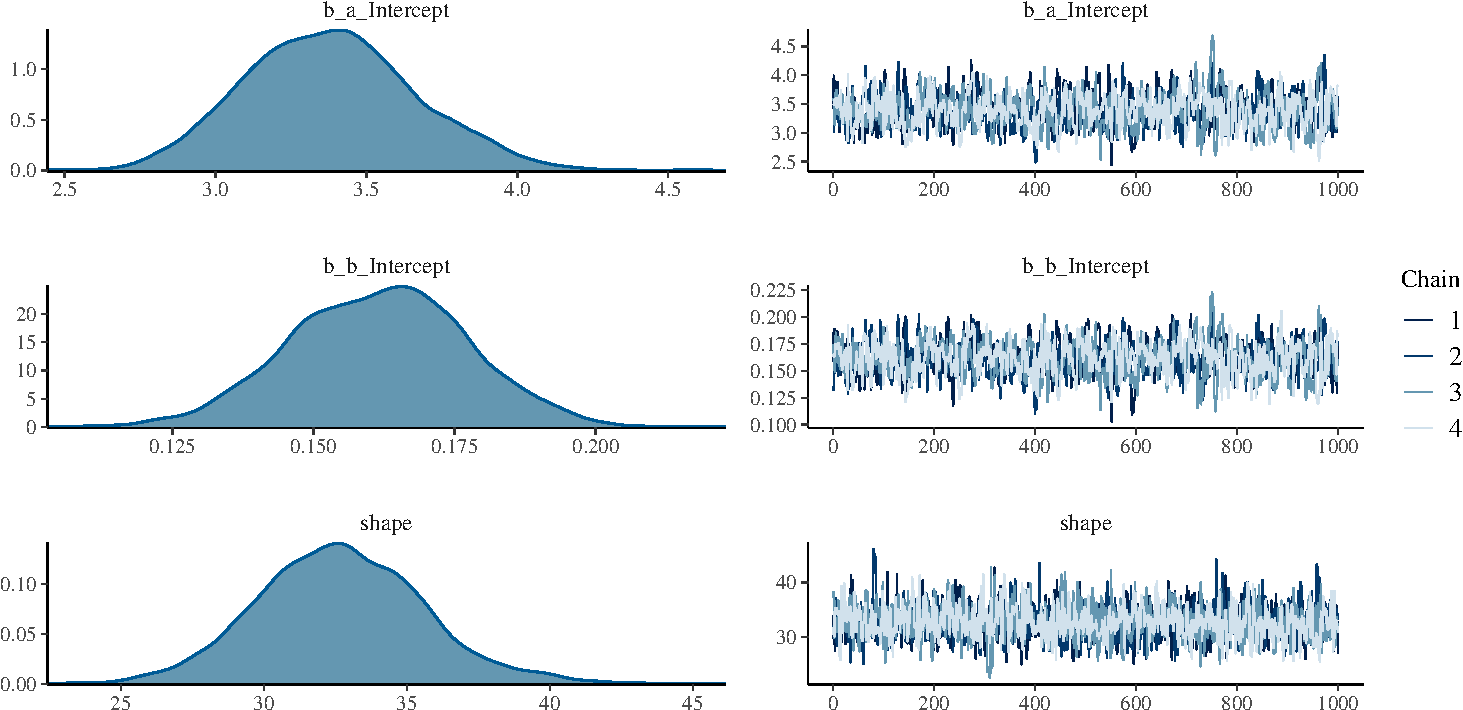
\includegraphics{intro_Bayes_files/figure-beamer/unnamed-chunk-19-1.pdf}

\end{frame}

\begin{frame}[fragile]{Model parameters}
\protect\hypertarget{model-parameters}{}

\tiny

\begin{Shaded}
\begin{Highlighting}[]
\KeywordTok{summary}\NormalTok{(fit_myx)}
\end{Highlighting}
\end{Shaded}

\begin{verbatim}
##  Family: gamma 
##   Links: mu = identity; shape = identity 
## Formula: titer ~ a * day * exp(-b * day) 
##          a ~ fgrade
##          b ~ fgrade
##    Data: MyxoTiter_sum (Number of observations: 149) 
## Samples: 4 chains, each with iter = 2000; warmup = 1000; thin = 1;
##          total post-warmup samples = 4000
## 
## Population-Level Effects: 
##             Estimate Est.Error l-95% CI u-95% CI Rhat Bulk_ESS Tail_ESS
## a_Intercept     3.38      0.29     2.86     3.96 1.01      795     1094
## a_fgrade3      -0.89      0.33    -1.56    -0.27 1.00      932     1459
## a_fgrade4      -1.38      0.30    -2.00    -0.83 1.00      824     1126
## a_fgrade5      -0.97      0.31    -1.61    -0.40 1.01      835     1141
## b_Intercept     0.16      0.02     0.13     0.19 1.01      792      964
## b_fgrade3      -0.06      0.02    -0.10    -0.03 1.00      821     1060
## b_fgrade4      -0.08      0.02    -0.11    -0.05 1.00      793      992
## b_fgrade5      -0.02      0.02    -0.05     0.02 1.01      800     1073
## 
## Family Specific Parameters: 
##       Estimate Est.Error l-95% CI u-95% CI Rhat Bulk_ESS Tail_ESS
## shape    32.71      2.96    27.19    39.03 1.00     1509     1718
## 
## Samples were drawn using sampling(NUTS). For each parameter, Bulk_ESS
## and Tail_ESS are effective sample size measures, and Rhat is the potential
## scale reduction factor on split chains (at convergence, Rhat = 1).
\end{verbatim}

\normalsize

Grade 1 (the intercept) looks more virulent than the others.

\end{frame}

\begin{frame}[fragile]{Interpreting the deterministic model}
\protect\hypertarget{interpreting-the-deterministic-model}{}

Our deterministic model takes the form \[
\mu_{titer}=a_{g}te^{-b_{g}t}
\] The parameters relate to the onset rapidity and the recovery rate for
each grade of the virus.

\begin{itemize}
\tightlist
\item
  \(a_g\) is the initial slope
\item
  \(1/b_g\) is the \(t\)-coordinate of the maximum.
\end{itemize}

\scriptsize

\begin{Shaded}
\begin{Highlighting}[]
\NormalTok{x <-}\StringTok{ }\KeywordTok{summary}\NormalTok{(fit_myx)}\OperatorTok{$}\NormalTok{fixed[,}\StringTok{"Estimate"}\NormalTok{]}
\NormalTok{myx_det <-}\StringTok{ }\ControlFlowTok{function}\NormalTok{(day, grade)\{}
\NormalTok{  a <-}\StringTok{ }\NormalTok{x[}\DecValTok{1}\NormalTok{] }\OperatorTok{+}\StringTok{ }\NormalTok{x[}\DecValTok{2}\NormalTok{]}\OperatorTok{*}\NormalTok{(grade}\OperatorTok{==}\DecValTok{3}\NormalTok{) }\OperatorTok{+}\StringTok{ }\NormalTok{x[}\DecValTok{3}\NormalTok{]}\OperatorTok{*}\NormalTok{(grade}\OperatorTok{==}\DecValTok{4}\NormalTok{) }\OperatorTok{+}\StringTok{ }\NormalTok{x[}\DecValTok{4}\NormalTok{]}\OperatorTok{*}\NormalTok{(grade}\OperatorTok{==}\DecValTok{5}\NormalTok{)}
\NormalTok{  b <-}\StringTok{ }\NormalTok{x[}\DecValTok{5}\NormalTok{] }\OperatorTok{+}\StringTok{ }\NormalTok{x[}\DecValTok{6}\NormalTok{]}\OperatorTok{*}\NormalTok{(grade}\OperatorTok{==}\DecValTok{3}\NormalTok{) }\OperatorTok{+}\StringTok{ }\NormalTok{x[}\DecValTok{7}\NormalTok{]}\OperatorTok{*}\NormalTok{(grade}\OperatorTok{==}\DecValTok{4}\NormalTok{) }\OperatorTok{+}\StringTok{ }\NormalTok{x[}\DecValTok{8}\NormalTok{]}\OperatorTok{*}\NormalTok{(grade}\OperatorTok{==}\DecValTok{5}\NormalTok{)}
\NormalTok{  a}\OperatorTok{*}\NormalTok{day}\OperatorTok{*}\KeywordTok{exp}\NormalTok{(}\OperatorTok{-}\NormalTok{b}\OperatorTok{*}\NormalTok{day)}
\NormalTok{\}}
\end{Highlighting}
\end{Shaded}

\end{frame}

\begin{frame}{Comparing the model to the data}
\protect\hypertarget{comparing-the-model-to-the-data}{}

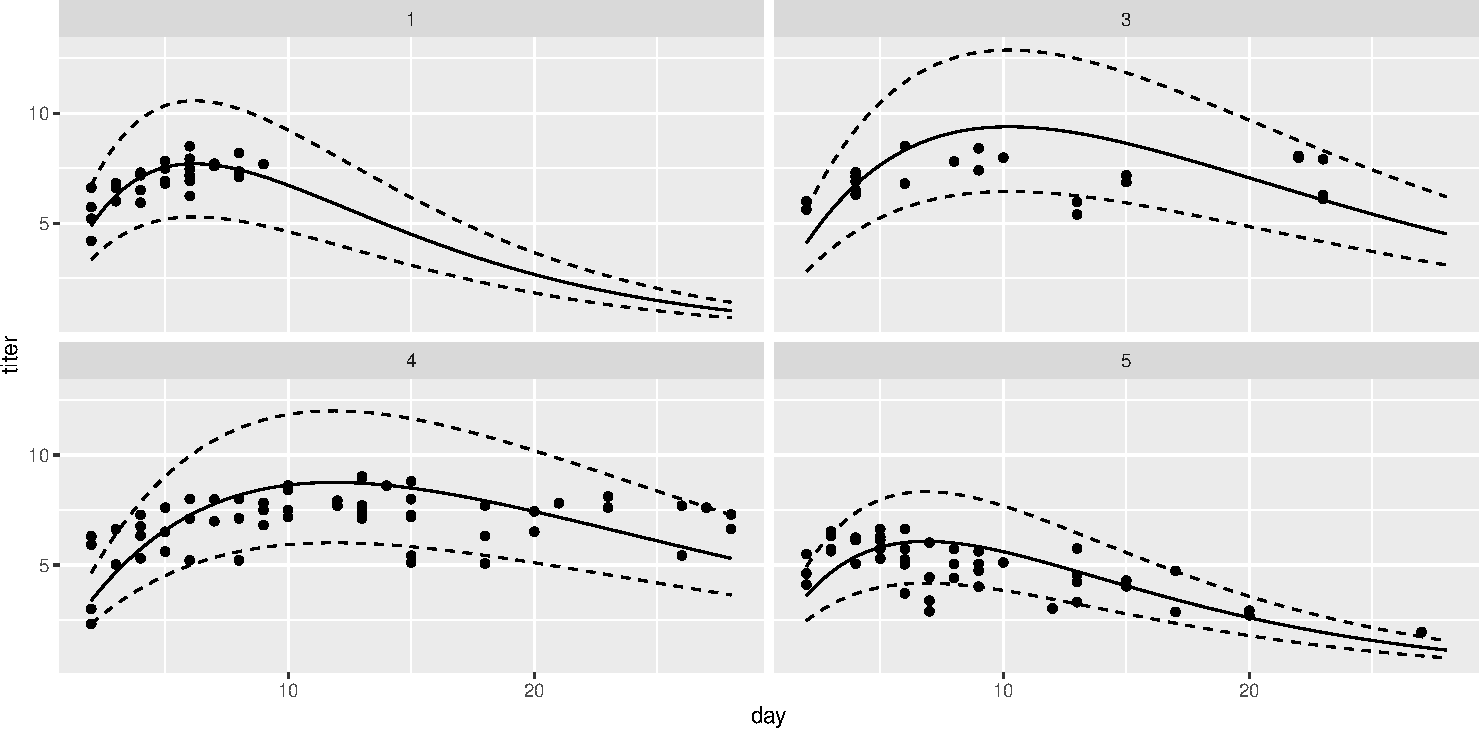
\includegraphics{intro_Bayes_files/figure-beamer/unnamed-chunk-22-1.pdf}

The code to create this plot is ugly, so it's not included on the slide.
It looks like the model does okay, but there might be some dynamics to
the virus in the second week of infection that the model misses.

Note that all the rabbits infected with grade 1 die before day 10.

\end{frame}

\begin{frame}[fragile]{Leave-one-out cross validation}
\protect\hypertarget{leave-one-out-cross-validation}{}

\begin{itemize}
\tightlist
\item
  For each observation, build a model excluding that observation.
\item
  Compute the log-likelihood of the excluded observation.
\item
  Combine all these log-likelihoods to assess the model.
\end{itemize}

\tiny

\begin{Shaded}
\begin{Highlighting}[]
\KeywordTok{loo}\NormalTok{(fit_myx, }\DataTypeTok{moment_match =} \OtherTok{TRUE}\NormalTok{)}
\end{Highlighting}
\end{Shaded}

\begin{verbatim}
## Warning: Some Pareto k diagnostic values are slightly high. See help('pareto-k-diagnostic') for details.
\end{verbatim}

\begin{verbatim}
## 
## Computed from 4000 by 149 log-likelihood matrix
## 
##          Estimate   SE
## elpd_loo   -278.8 16.6
## p_loo        16.1  3.2
## looic       557.7 33.3
## ------
## Monte Carlo SE of elpd_loo is 0.1.
## 
## Pareto k diagnostic values:
##                          Count Pct.    Min. n_eff
## (-Inf, 0.5]   (good)     145   97.3%   408       
##  (0.5, 0.7]   (ok)         4    2.7%   272       
##    (0.7, 1]   (bad)        0    0.0%   <NA>      
##    (1, Inf)   (very bad)   0    0.0%   <NA>      
## 
## All Pareto k estimates are ok (k < 0.7).
## See help('pareto-k-diagnostic') for details.
\end{verbatim}

\end{frame}

\begin{frame}[fragile]{How does a \texttt{glm} do?}
\protect\hypertarget{how-does-a-glm-do}{}

Try a quadratic in \texttt{day} for the deterministic part of the model.
\tiny

\begin{Shaded}
\begin{Highlighting}[]
\NormalTok{myx_glm <-}\StringTok{ }\KeywordTok{glm}\NormalTok{(titer}\OperatorTok{~}\KeywordTok{poly}\NormalTok{(day,}\DecValTok{2}\NormalTok{)}\OperatorTok{*}\NormalTok{fgrade, }
               \DataTypeTok{family =} \KeywordTok{Gamma}\NormalTok{(}\DataTypeTok{link =} \StringTok{"identity"}\NormalTok{), }\DataTypeTok{data=}\NormalTok{MyxoTiter_sum)}
\KeywordTok{summary}\NormalTok{(myx_glm)}
\end{Highlighting}
\end{Shaded}

\begin{verbatim}
## 
## Call:
## glm(formula = titer ~ poly(day, 2) * fgrade, family = Gamma(link = "identity"), 
##     data = MyxoTiter_sum)
## 
## Deviance Residuals: 
##      Min        1Q    Median        3Q       Max  
## -0.72518  -0.07252   0.02296   0.10848   0.32272  
## 
## Coefficients:
##                       Estimate Std. Error t value Pr(>|t|)
## (Intercept)             4.2571     3.1725   1.342    0.182
## poly(day, 2)1         -62.8351    67.8145  -0.927    0.356
## poly(day, 2)2         -40.6835    29.9023  -1.361    0.176
## fgrade3                 2.7455     3.1820   0.863    0.390
## fgrade4                 2.4561     3.1760   0.773    0.441
## fgrade5                 0.4325     3.1745   0.136    0.892
## poly(day, 2)1:fgrade3  64.4313    67.8661   0.949    0.344
## poly(day, 2)2:fgrade3  37.6151    30.1050   1.249    0.214
## poly(day, 2)1:fgrade4  70.0160    67.8333   1.032    0.304
## poly(day, 2)2:fgrade4  34.0673    29.9390   1.138    0.257
## poly(day, 2)1:fgrade5  50.5914    67.8263   0.746    0.457
## poly(day, 2)2:fgrade5  40.0406    29.9247   1.338    0.183
## 
## (Dispersion parameter for Gamma family taken to be 0.02619576)
## 
##     Null deviance: 10.6424  on 148  degrees of freedom
## Residual deviance:  4.1168  on 137  degrees of freedom
## AIC: 454.09
## 
## Number of Fisher Scoring iterations: 6
\end{verbatim}

\end{frame}

\begin{frame}{The GLM fits well but is less interpretable}
\protect\hypertarget{the-glm-fits-well-but-is-less-interpretable}{}

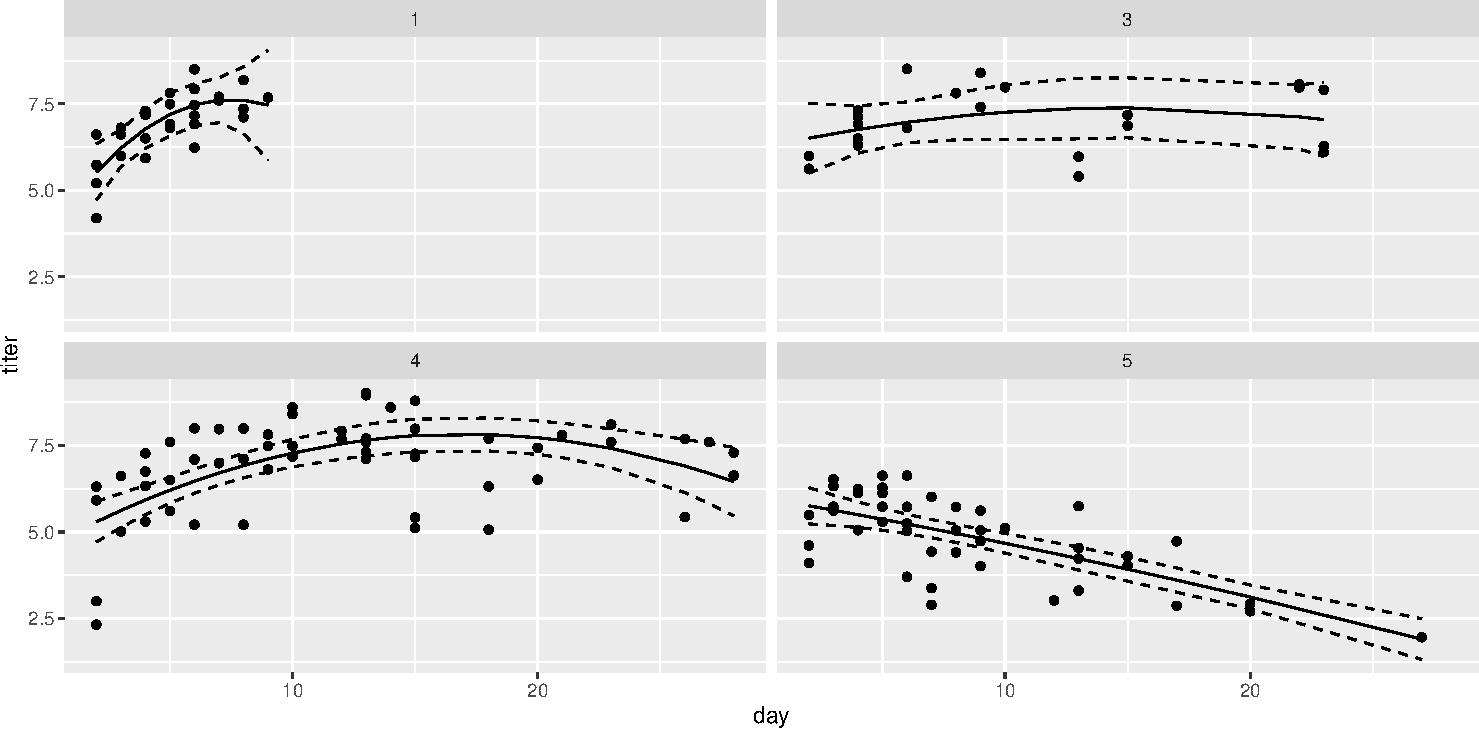
\includegraphics{intro_Bayes_files/figure-beamer/unnamed-chunk-25-1.pdf}

If we just want to interpolate, this seems like a good model.

\end{frame}

\begin{frame}[fragile]{AIC}
\protect\hypertarget{aic}{}

\texttt{brms} doesn't support AIC, but we can compute it if we want to.
\texttt{AIC\_maybe} of the Bayesian model looks reasonable - it's
similar to the \texttt{looic} and not too far from the AIC for the
\texttt{glm}, which is perhaps overfit. I did have to build it by hand,
the \texttt{numeric(0)} means there isn't a \texttt{brmsfit} method for
\texttt{AIC}.

\scriptsize

\begin{Shaded}
\begin{Highlighting}[]
\KeywordTok{AIC}\NormalTok{(myx_glm)}
\end{Highlighting}
\end{Shaded}

\begin{verbatim}
## [1] 454.0936
\end{verbatim}

\begin{Shaded}
\begin{Highlighting}[]
\KeywordTok{AIC}\NormalTok{(fit_myx)}
\end{Highlighting}
\end{Shaded}

\begin{verbatim}
## numeric(0)
\end{verbatim}

\begin{Shaded}
\begin{Highlighting}[]
\NormalTok{llMyx <-}\StringTok{ }\KeywordTok{log_lik}\NormalTok{(fit_myx)}
\CommentTok{# ?brms::logLik.brmsfit}
\NormalTok{nllMyx <-}\StringTok{ }\OperatorTok{-}\KeywordTok{sum}\NormalTok{(}\KeywordTok{colMeans}\NormalTok{(llMyx))}
\NormalTok{(AIC_maybe <-}\StringTok{ }\DecValTok{2}\OperatorTok{*}\NormalTok{nllMyx}\DecValTok{-2}\OperatorTok{*}\KeywordTok{dim}\NormalTok{(fit_myx}\OperatorTok{$}\NormalTok{data)[}\DecValTok{2}\NormalTok{])}
\end{Highlighting}
\end{Shaded}

\begin{verbatim}
## [1] 532.6945
\end{verbatim}

\end{frame}

\begin{frame}{References}
\protect\hypertarget{references}{}

\hypertarget{refs}{}
\leavevmode\hypertarget{ref-bolker}{}%
Bolker, Benjamin M. 2008. \emph{Ecological Models and Data in R}.
Princeton University Press.

\leavevmode\hypertarget{ref-brms}{}%
Bürkner, Paul-Christian. 2018. ``Advanced Bayesian Multilevel Modeling
with the R Package brms.'' \emph{The R Journal} 10 (1): 395--411.
\url{https://doi.org/10.32614/RJ-2018-017}.

\end{frame}

\end{document}
